\documentclass[12pt]{article}
\usepackage{amsmath, amssymb, amsthm, tikz, pgf, graphicx}
\usetikzlibrary{arrows,automata}
\usepackage[latin1]{inputenc}

\begin{document}

\title{Class Handout: Word Graphs}
\author{Lawrence Wu}
\date{November 22, 2014}

\maketitle

\section{Useful Ideas}
It is helpful but not necessary to know some fundamentals of computer programming, algorithms/data structures, runtime/space analysis, and graph theory. Bolded words are defined in the glossary at the end. 

\section{Overview}
We will learn techniques for tasks such as autocomplete/dictionary lookup, finding keywords/\textbf{strings} in a document, or imitating someone's speech patterns. The key intuition will be thinking of characters as \textbf{transitions} between \textbf{states}. \\

An electronic copy of this handout is available at https://raw.githubusercontent.com/llwu/ESP-teaching-materials/master/Splash-2014-Word-Graphs/handout.pdf (this link has been e-mailed to all students shortly before the class starts for those who prefer to read that way).

\section{The Normal Way to Store a String}
The way a computers memory is built is as a bunch of \textbf{bits}: devices that we can turn on/off or read whether it is on/off. We organize the bits into groups of $8$ each (called \textbf{bytes}), and label each group with a \textbf{memory address}, much like a row of houses. \\

\includegraphics{memdiagram.png} \\

Since a bit can represent $2$ different values, a byte can represent $2^8 = 256$ different values. So there's no way way we would be represent an entire word in a byte, since there are definitely more than $256$ words. But there aren't that many distinct characters (things like upper/lowercase letters, numbers, punctuation), so we could represent each character in a byte! So here's how we'll write a word/sentence/text: we'll reserve a block of memory, and write the first letter in the first byte, the second letter in the second byte, and so on. Then we'll put a "\textbf{null terminator}" at the end, which is a special character (represented by all bits being off, or the number $0$, also written as '\textbackslash 0') that tells the computer where to stop reading. So when we need to read a word/sentence/text, we need the address of the first byte, so we can just read off the letters starting from there one by one until we reach '\textbackslash 0', then we stop. An address can be stored as a sequence of $4$ bytes (using the binary number system to represent $0$ to $2^{32} - 1 = 4294967295$). So we can store a list of addresses (if we know where the list starts and how long the list is) in sequence, like a phone book. This is the basic way to store a dictionary of words: store the words+definitions throughout memory, and store a list of their addresses. This works much like a dictionary in real life, and lookup is done much the same way (go to the middle word, then see if we need to go to the right or the left, takes some small amount of effort). However, inserting/deleting words is a pain - remember how memory is organized like a row of houses? Imagine trying to build a new house between two existing houses - you'd have to move a bunch of other houses over first!

\section{Tries}
Here's an idea: Think of the large real-life dictionaries that have indents for words starting with 'A', words starting with 'B', etc. If we organized our words this way in our computer's memory, we could save a little bit of effort from lookups. This could be done by turning our dictionary into a list of $26$ addresses, each for a subdictionary (each represents words starting with a specific letter). Notice that with smaller subdictionaries, it would also take less work to insert/delete! So this is certainly an improvement. But why stop there when we can keep going? We could make each subdictionary link to another list of subdictionaries, and so on until there are no more words! So the 'A' subdictionary would link to the 'AA', 'AB', ... , 'AZ' subdictionaries, and each of those would link to more ('AAA', 'AAB', etc). The \textbf{data structure} that we have created will look something like this: \\

\includegraphics{triediagram.png} \\

There's quite a bit going on in this diagram, so let's break it down:
\begin{itemize}
  \item Each block of memory (shown as a house) is called a "\textbf{node}", and it represents a subdictionary of words starting with some \textbf{prefix} (Note that prefix has a different meaning in computer science than in English - any beginning of the word counts as a prefix! For example, "AA" is a prefix of "AARDVARK"). It stores two addresses: a subdictionary address pointing to a list of $26$ "child" nodes, and a definition address pointed to a null-terminated string containing the definition of the word formed so far. To save room, I didn't draw all $26$ child nodes of each node, and I didn't draw $8$ houses for the $8$ ($4$ bytes for each stored address) bytes that each node takes (I did, however make the example addresses $8$ apart in the row of houses).
  \item Generally, computers reserve some byte that programs aren't allowed to write/read. The address of this byte (usually $0$) is denoted \textbf{Null}, and is usually used to denote that something doesn't exist. For example, if we can't continue adding letters to a word, we'll set that node's subdictionary \textbf{pointer} to Null and stop making more subdictionaries. Also, if the prefix denoted by some node is not a word, then we'll set its definition pointer to Null because we can't write a definition.
  \item To lookup a word, start at the top node (called the "root"), and read its letters one by one, going to the correct child node for each letter. This will take us to the node representing our word, and we can just return the definition from the definition pointer, if it exists. To delete a word, go to the node the same way we did just now, and set the definition pointer to Null. To insert a word, go to the node the same way we did just now, make a new definition, and set the definition pointer to our new definition's address (we might have to create some new nodes along the way but it doesn't take the computer much effort). These operations are all quite efficient.
  \item We can make the nodes as big as we like, if we want to store more \textbf{auxiliary data} that would be helpful to us (this is called \textbf{augmenting} the data structure). For example, at each node we can store the number of words included in the subdictionary represented by it. If we do this, we can show the number of matches for Autocomplete (just go to the node represented by whatever the user has typed in, and read off the number of words). Also, if the number of words in the subdictionary reaches $0$, we can free up the spaces used by the subdictionary pointer and set it to Null to save space. Another augmentation we can put is, for each node, a pointer to a list of most common autocomplete suggestions. Then, as a user types each letter, we can move to the correct node and update our list of suggestions.
\end{itemize}
Many other minor improvements can be made as well.

\section{Graphs}
I did call this class Word \textbf{Graphs} after all. Now that we have the intuition about tries, it's a good time to define what a graph is in the context of computer science. We aren't talking about the kind of graph covered in middle/high school which show data or plot a function. What "graph" means here is a set of \textbf{vertices} (a.k.a. nodes) and \textbf{edges}, each of which connects a vertex to another vertex. The structure should feel somewhat familiar; indeed, a trie looks a lot like a graph - the nodes of the trie look like vertices and the pointers look like edges. In fact, our definition of graph is quite vague and general, and therefore a graph could represent many things (e.g. social networks, computer networks, electrical/water systems, maps), making graphs very useful in real-life applications (the fact that they're also interesting in theory is a bonus!). For the rest of this class we will study mathematical models of words that look like graphs (in particular they will look like \textbf{directed graphs}, which are graphs in which each edge has a direction i.e. it points from one vertex to another).

\section{Introduction to automata}
Let's begin with a sample problem. How many ways can I write $100$ letters without ever writing "CAT"? Without writing "BABOON"? Without writing either? This problem is somewhat related to the "infinite monkey theorem" (from Wikipedia, "if a monkey randomly types letters forever, it will almost surely type a given text, such as the complete works of William Shakespeare"). Unfortunately, for longer given texts, the monkey will have to type quite a lot of characters before it is likely that they have typed the given text. We will see a bit of this numerical trend in solving our problem. \\

\textit{(spoilers ahead)} \\

\textit{(spoilers ahead)} \\

OK, it's not so hard to count the ways to write $100$ letters with no restriction. That would be $26^{100} \approx 3.142931\times 10^{141}$, since for each of the $100$ letters we have $26$ choices. Equivalently, writing $100$ letters is like walking $100$ steps on the following graph ("$s$" denotes start, and in the picture we abbreviate $26$ edges from $s$ to $s$ with a single $A-Z$ edge from $s$ to $s$):

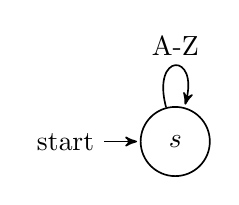
\begin{tikzpicture}[->,>=stealth',shorten >=1pt,auto,node distance=2.8cm,
                    semithick]
  \tikzstyle{every state}=[fill=white,draw=black,text=black]

  \node[initial,state] (A)                     {$s$};

  \path (A) edge  [loop above]                 node {A-Z} (A);
\end{tikzpicture}

Can we make similar graph that shows the added restriction of not writing "CAT"? It turns out that we can:

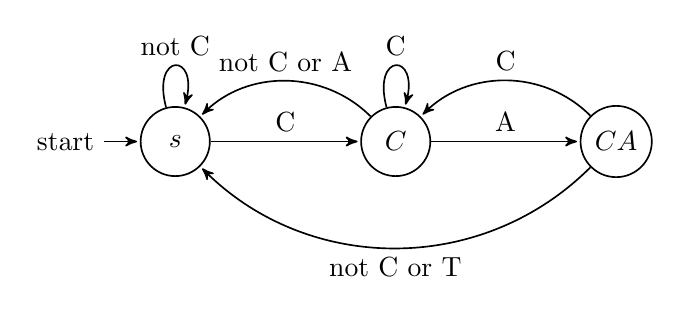
\begin{tikzpicture}[->,>=stealth',shorten >=1pt,auto,node distance=2.8cm,
                    semithick]
  \tikzstyle{every state}=[fill=white,draw=black,text=black]

  \node[initial,state] (A)                     {$s$};
  \node[state]         (B)        [right of=A] {$C$};
  \node[state]         (C)        [right of=B] {$CA$};

  \path (A) edge                               node {C} (B)
            edge [loop above]                  node {not C} (A)
        (B) edge                               node {A} (C)
            edge [loop above]                  node {C} (B)
            edge [out=135,in=45]               node [above] {not C or A} (A)
        (C) edge [out=135,in=45]               node [above] {C} (B)
            edge [out=225,in=315]              node [below] {not C or T} (A);
\end{tikzpicture}

Now we explain how this graph works. Each state represents our progress towards spelling "CAT". $s$ represents no progress. So writing $C$ at state $s$ transitions us to state $C$, writing $A$ at state $C$ transitions us to state $CA$, and writing $T$ at state $CA$ is disallowed, because then we would spell out "CAT". Similarly, writing $C$ at states $C$ or $CA$ transitions us to state $C$. Anything else gets rid of our progress, so it brings us back to state $s$. Now, each $100$ letter word without "CAT" corresponds to a $100$-step walk on this graph. Counting these takes maths knowledge outside the scope of this class, so don't worry about understanding this, but basically taking the adjacency matrix to the $100$-th power gives an answer of about $3.125453\times 10^{141}$ (which means there's only about a $0.5561\%$ chance that a random $100$-letter word contains "CAT"!). We can actually get a closed form of approximately $25.9985^n$ ways to write $n$ letters without writing "CAT" by diagonalization. So we'd have to write about $12000$ letters before we've had a $50\%$ chance of writing "CAT".

\newpage

Now that we've seen an example, see if you can figure out the graph for "BABOON", and the combined graph for "BABOON" and "CAT". The answer for "BABOON" is on the next page (the flip side of this page). By the way, the kind of "graphs" we're constructing are also called \textbf{automata}, a.k.a. \textbf{state machines}. They also have the properties "deterministic", because the walk is uniquely determined by the letters we write, and "finite", because there are finitely many states. So we get the intimidating name "deterministic finite automaton (DFA)"/"deterministic finite state machine".

\textit{(check next page for spoilers)}

\newpage

Answers:

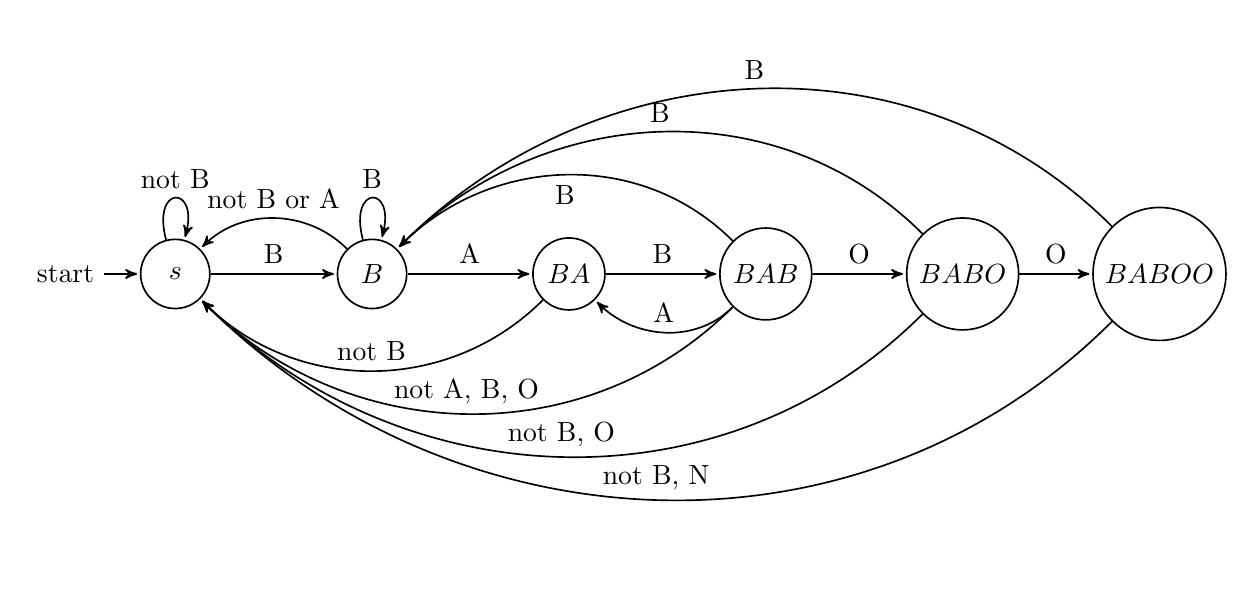
\begin{tikzpicture}[->,>=stealth',shorten >=1pt,auto,node distance=2.5cm,
                    semithick]
  \tikzstyle{every state}=[fill=white,draw=black,text=black]

  \node[initial,state] (A)                     {$s$};
  \node[state]         (B)        [right of=A] {$B$};
  \node[state]         (C)        [right of=B] {$BA$};
  \node[state]         (D)        [right of=C] {$BAB$};
  \node[state]         (E)        [right of=D] {$BABO$};
  \node[state]         (F)        [right of=E] {$BABOO$};

  \path (A) edge                               node {B} (B)
            edge [loop above]                  node {not B} (A)
        (B) edge                               node {A} (C)
            edge [loop above]                  node {B} (B)
            edge [out=135,in=45]               node [above] {not B or A} (A)
        (C) edge                               node {B} (D)
            edge [out=225,in=315]              node [above] {not B} (A)
        (D) edge                               node {O} (E)
            edge [out=225,in=315]              node [above] {A} (C)
            edge [out=135,in=45]               node [below] {B} (B)
            edge [out=225,in=315]              node [above] {not A, B, O} (A)
        (E) edge                               node {O} (F)
            edge [out=135,in=45]               node [above] {B} (B)
            edge [out=225,in=315]              node [above] {not B, O} (A)
        (F) edge [out=135,in=45]               node [above] {B} (B)
            edge [out=225,in=315]              node [above] {not B, N} (A);
\end{tikzpicture}
The same advanced math methods as before give an answer of $3.14293\times 10^{141}$ ways to write $100$ letters without writing "BABOON" - this is less than a $0.0001\%$ chance that $100$ random letters will contain "BABOON"! The closed form answer is approximately $25.9999999158^n$ ways to write $n$ letters without writing "BABOON", which means we'd have to write about $210000000$ letters to have a $50\%$ chance of writing "BABOON"! So much for writing Shakespeare!


\section{Automata application to string matching}
What can we take away from the previous section and apply to computer science? We turned a word into a graph that represents all the ways to write letters without writing the word. It turns out that although this process is tedious to do by hand, but computers can do it efficiently (we will take this for granted here, since the details are a bit gnarly). We can apply this to find a keyword/keywords inside a document. Process the keyword/keywords into its automata. Then go through each letter of the document, simulating a step on the automata. If we're ever unable to make the step, it must be because we spelled out the word, so we have a match at that location. Fun fact: this method is called the "Aho-Corasick Algorithm" and it is used in the Unix command "fgrep". One thing to note about this method is that once we've processed the keyword, we won't have to process it again until the keyword changes, since we already have the automata. This makes the algorithm good for searching many documents with the same set of keywords. \\

There exists a more advanced method (which also is applicable to different situations) covered in the "Further Reading" section, called the suffix automaton. It is an automaton recognizing all suffixes of a string. Let's take it for granted that this is efficiently constructable. Since the substring of a string are exactly the prefixes of one of its suffixes, a keyword is a substring if and only if it is a valid walk on the suffix automaton. So if we do many CTRL+F searches on the same document, this method is very efficient since we can just make the suffix automaton of the document once, and run every query on this automaton.

\section{Markov chain text generation}
Let's change the tune. We've had letters transitioning into the next letters until now. What about words transitioning into words? We will show how to model a person's speech this way. \\

A naive way to model a person's speech is to count up all their usages of each word, and randomly spit out words based on those counts (for example, if I say "cat" 3 times and "dog" 2 times, then the naive model would spit out "cat" $60\%$ of the time and dog $40\%$ of the time). If we tried this method, we would immediately see that it would result in incredibly poor grammar. So let's modify our model so that we now assume our person's next word is influenced by their previous $k$ words. This is called a $k$-gram model. Our naive method would be a $0$-gram model (as an exercise for the intuition, what do you think changing $k$ does?). Let's make an illustrative example of a $2$-gram model. Suppose these are these are the quotes you have to work with: \\
"I like pie." \\
"I like pie." \\
"I like pie." \\
"I like cats." \\
The state of our system is the last two words used, and the transitions are given by adding the next words. The initial state is "","" and at this state it seems we always say "I" next, so we add a $100\%$ chance transition (labeled with the word "I") to the state "", "I". Similarly, at this state, it seems we always say "like" next, so we add a $100\%$ chance transition (labeled with the word "like") to the state "I", "like". At this point, we've reached a crossroads. It seems we say "pie" next 3/4 times, so we add a  $75\%$ chance transition (labeled with the word "pie") to the state "like", "pie" as well as a $25\%$ chance transition (labeled with the word "cats") to the state "like", "cats". At either of these states, there is a $100\%$ chance of ending the sentence, so we can add a special transition there. Now our graph (the mathematical model it represents is called a "Markov chain") looks like this: \\

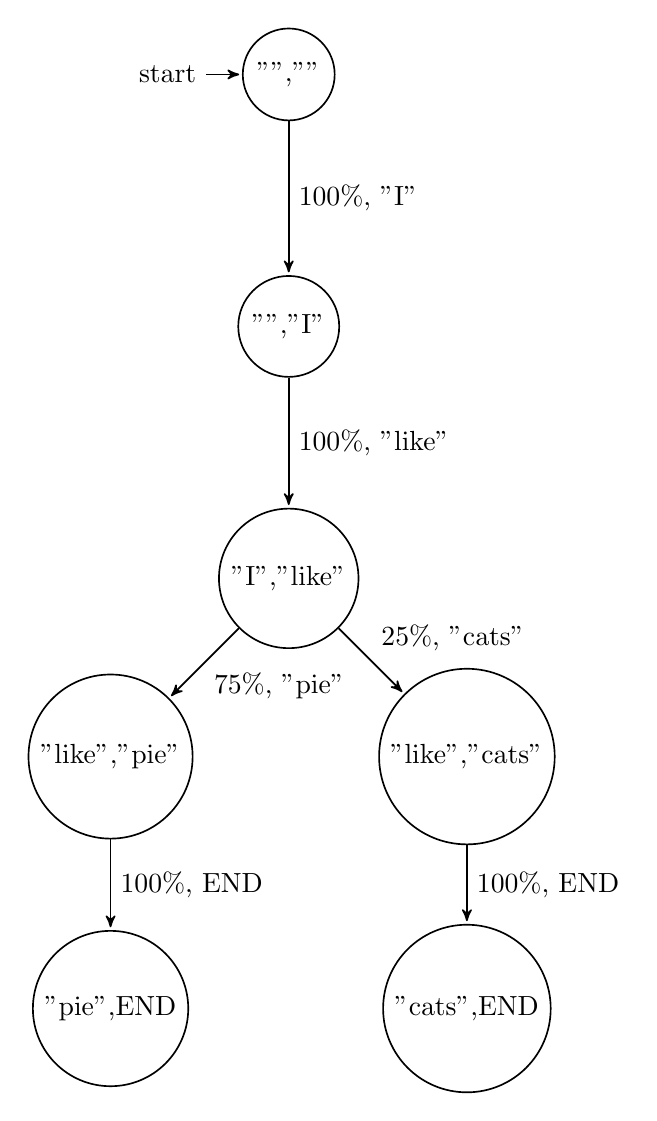
\begin{tikzpicture}[->,>=stealth',shorten >=1pt,auto,node distance=3.2cm,
                    semithick]
  \tikzstyle{every state}=[fill=white,draw=black,text=black]

  \node[initial,state] (A)                           {"",""};
  \node[state]         (B)        [below of=A]       {"","I"};
  \node[state]         (C)        [below of=B]       {"I","like"};
  \node[state]         (D)        [below left of=C] {"like","pie"};
  \node[state]         (E)        [below right of=C] {"like","cats"};
  \node[state]         (F)        [below of=D]       {"pie",END};
  \node[state]         (G)        [below of=E]       {"cats",END};

  \path (A) edge                               node {$100\%$, "I"}    (B)
        (B) edge                               node {$100\%$, "like"} (C)
        (C) edge                               node {$75\%$, "pie"}   (D)
            edge                               node {$25\%$, "cats"}  (E)
        (D) edge                               node {$100\%$, END}    (F)
        (E) edge                               node {$100\%$, END}    (G);
\end{tikzpicture}

The Markov chains for more complex data look more interesting. Although they are tedious to write by hand, computers can build Markov chain models efficiently. I've uploaded example code to https://raw.githubusercontent.com/llwu/ESP-teaching-materials/master/Splash-2014-Word-Graphs/MarkovDemo.cpp so that those who know some C++ could check out how to do it. To generate random sentences from this Markov chain, we just simulate walking randomly from the initial state (when we reach a crossroads, pick a random transition such that the probability that a transition is picked is equal to its label probability). \\ \\
Examples of Markov chain usage in popular culture: \\
http://kingjamesprogramming.tumblr.com \\
http://what-would-i-say.com/

\section{Further Reading}
If you liked the material of the class, you may later want to study string algorithms, automata theory, linear algebra, and probability theory. Some of following readings go more into detail about what we learned here, some go into different but related material. All are quite advanced: \\

\textit{http://e-maxx.ru/algo/suffix\_automata} (Russian suffix automaton tutorial, read with http://translate.yandex.com/translate)

\textit{https://genomics.soe.ucsc.edu/sites/default/files/smallest\_automaton1985.pdf} (original paper on suffix automata)

\textit{"Jewels of Stringology"} by Crochemore (book)

\textit{http://en.wikipedia.org/wiki/Adjacency\_matrix} (a connection between graph theory and linear algebra, see also "spectral graph theory")

\textit{http://en.wikipedia.org/wiki/Matrix\_diagonalization}

\textit{http://en.wikipedia.org/wiki/Markov\_chain}
\section{Glossary}
\textbf{augmenting} - adding auxiliary data to a data structure\\ \\
\textbf{automata} - see state machine\\ \\
\textbf{auxiliary data} - extra data fields that make computations convenient\\ \\
\textbf{bits} - basic building block of memory, on/off, 1/0\\ \\
\textbf{bytes} - 8 bits\\ \\
\textbf{data structure} - data organized in some efficient way\\ \\
\textbf{directed graphs} - graph in which every edge has a direction (to some vertex from another vertex)\\ \\
\textbf{edges} - something connecting two vertices\\ \\
\textbf{graphs} - set of vertices and edges\\ \\
\textbf{memory address} - location of a byte in memory\\ \\
\textbf{node} - vertex\\ \\
\textbf{null} - illegal memory address that signifies that something doesn't exist\\ \\
\textbf{null terminator} - signifies end of a null terminated string\\ \\
\textbf{pointer} - variable whose value is an address\\ \\
\textbf{prefix} - beginning of a string \\ \\
\textbf{state machines} - abstract machine that can transition between states\\ \\
\textbf{states} - the information about the status of a system that we care about\\ \\
\textbf{strings} - sequences of characters\\ \\
\textbf{transitions} - going from one state to another \\ \\
\textbf{vertices} - basic units of a graph

\end{document}
